\documentclass[a4paper,12pt]{extarticle}
\usepackage{geometry}
\usepackage[T1]{fontenc}
\usepackage[utf8]{inputenc}
\usepackage[english,russian]{babel}
\usepackage{amsmath}
\usepackage{amsthm}
\usepackage{amssymb}
\usepackage{fancyhdr}
\usepackage{setspace}
\usepackage{graphicx}
\usepackage{colortbl}
\usepackage{tikz}
\usepackage{pgf}
\usepackage{subcaption}
\usepackage{listings}
\usepackage{indentfirst}
\usepackage[
backend=biber,
style=numeric,
maxbibnames=99
]{biblatex}
\addbibresource{refs.bib}
\usepackage[colorlinks,citecolor=blue,linkcolor=blue,bookmarks=false,hypertexnames=true, urlcolor=blue]{hyperref} 
\usepackage{indentfirst}
\usepackage{mathtools}
\usepackage{booktabs}
\usepackage[flushleft]{threeparttable}
\usepackage{tablefootnote}

\usepackage{chngcntr} % нумерация графиков и таблиц по секциям
\counterwithin{table}{section}
\counterwithin{figure}{section}

\graphicspath{{graphics/}}%путь к рисункам

\makeatletter
% \renewcommand{\@biblabel}[1]{#1.} % Заменяем библиографию с квадратных скобок на точку:
\makeatother

\geometry{left=2.5cm}% левое поле
\geometry{right=1.0cm}% правое поле
\geometry{top=2.0cm}% верхнее поле
\geometry{bottom=2.0cm}% нижнее поле
\setlength{\parindent}{1.25cm}
\renewcommand{\baselinestretch}{1.5} % междустрочный интервал


\newcommand{\bibref}[3]{\hyperlink{#1}{#2 (#3)}} % biblabel, authors, year
\addto\captionsrussian{\def\refname{Список литературы (или источников)}} 

\renewcommand{\theenumi}{\arabic{enumi}}% Меняем везде перечисления на цифра.цифра
\renewcommand{\labelenumi}{\arabic{enumi}}% Меняем везде перечисления на цифра.цифра
\renewcommand{\theenumii}{.\arabic{enumii}}% Меняем везде перечисления на цифра.цифра
\renewcommand{\labelenumii}{\arabic{enumi}.\arabic{enumii}.}% Меняем везде перечисления на цифра.цифра
\renewcommand{\theenumiii}{.\arabic{enumiii}}% Меняем везде перечисления на цифра.цифра
\renewcommand{\labelenumiii}{\arabic{enumi}.\arabic{enumii}.\arabic{enumiii}.}% Меняем везде перечисления на цифра.цифра

\begin{document}
\begin{titlepage}
\newpage

{\setstretch{1.0}
\begin{center}
ПРАВИТЕЛЬСТВО РОССИЙСКОЙ ФЕДЕРАЦИИ\\
ФГАОУ ВО НАЦИОНАЛЬНЫЙ ИССЛЕДОВАТЕЛЬСКИЙ УНИВЕРСИТЕТ\\
«ВЫСШАЯ ШКОЛА ЭКОНОМИКИ»
\\
\bigskip
Факультет компьютерных наук\\
Образовательная программа «Прикладная математика и информатика»
\end{center}
}

\vspace{2em}
% УДК ХХХХХ
\vspace{5em}

\begin{center}
%Выберите какой у вас проект
% {\bf Отчет об исследовательском проекте на тему:}\\
{\bf Отчет о программном проекте на тему:}\\
{\bf Хэширование с учётом энтропии}
\end{center}

\vspace{2em}

{\bf Выполнил: \vspace{2mm}}

{\setstretch{1.0}
\begin{tabular}{l@{\hskip 1.5cm}c@{\hskip 1.5cm}c}
студент группы БПМИ215 & & \\
Тереничев Дмитрий Александрович & \rule{3.5cm}{0.15mm}  &  \rule{3.5cm}{0.15mm} \vspace{-2mm} \\
 & \tiny{(подпись)}  & \tiny{(дата)} \\
\end{tabular}}

\vspace{1em}
{\bf Принял руководитель проекта: \vspace{2mm}}

{\setstretch{1.0}
\begin{tabular}{l@{\hskip 1.5cm}l}
Коновалов Дмитрий Львович\\
Научный сотрудник (что здесь правильно написать?)\\
Факультета компьютерных наук НИУ ВШЭ \vspace{10mm}\\
\rule{4cm}{0.15mm}  &  \rule{4cm}{0.15mm} \vspace{-2mm}\\
{\hskip 1.5cm}\tiny{(подпись)} & {\hskip 1.5cm}\tiny{(дата)} \\
\end{tabular}}

\vspace{\fill}

\begin{center}
Москва 2023
\end{center}

\end{titlepage}% это титульный лист - выберите подходящий вам из имеющихся в проекте вариантов
\newpage
\setcounter{page}{2}

{
	\hypersetup{linkcolor=black}
	\tableofcontents
}

\newpage

\newpage
\section{Аннотация}   % this is how to use russian
Курсовой проект представляет собой реализацию метода хэширования с учётом энтропии в СУБД ClickHouse. Пользователи СУБД используют хэширование для ускорения поиска данных, для проверок целостности данных, для распределения данных между серверами, поэтому его скорость важна для пользователей. Классические алгоритмы хэширования, хоть и хорошо оптимизированы по скорости работы, для этих оптимизаций никак не используют информацию, содержащуюся в самих хэшируемых данных. Однако, если мы знаем особенности данных, которые будут хэшироваться, то можем использовать эти знания для ускорения хэширования. 

Суть используемого мной метода состоит в том, что бы хэшировать не все строки, а только символы на определённых позициях в них обычной хэш-функцией. Функция обучается один раз на наборе строк, то есть выбирает номера позиций символов в строках, наиболее сильно их различающие. Далее эти выбранные позиции используются для хэширования уже других строк, вычисляя обычный хэш от их подпоследовательностей, состоящих из символов на ранее выбранных позициях. 

Оптимизация заключается в уменьшении размера хэшируемой строки. Например, для строк $aa, ab, ac$ при хэшировании имеет смысл использовать только второй символ, игнорируя первый, т.к. первый символ никак не различает строки. Другой пример: если мы имеем массив url-адресов, то первые 4 символа в них бесполезны для хэширования, поскольку они все равны $http$. 

% \addcontentsline{toc}{section}{Аннотация}

\section{Ключевые слова}
Базы данных, системы управления базами данных, СУБД, хэш-функции, хэширование с учётом энтропии, оптимизация хэширования, ускорение хэширования.
\pagebreak

% TODO Переименовать разделы по-нормальному, согласно именно моей теме!

\section{Введение}
\subsection{Описание предметной области}

В СУБД существуют функции хеширования, они позволяют пользователям проще и быстрее работать с данными. В рамках своего курсового проекта я реализовал метод хэширования с учётом энтропии в ClickHouse -- колоночной СУБД с открытым исходным кодом, написанной на языке C++.

\subsection{Постановка задачи}

Задача -- внедрить в ClickHouse функции, осуществляющие обучение модели на наборе строк и хэширующие, возможно, другой набор строк, использую данные, полученные в результате обучения. Первая функция за полиномиальное время определяет, какие позиции в строках-элементах данных несут больше информации о данных, а вторая -- используя посчитанные первой функцией номера позиций, выбирает только нужные символы из строк и передаёт их в хэш-функцию, которой может являться любая из существующих.

\subsection{Актуальность и значимость}

К данному моменту разработано большое количество разнообразных хэш-функций, в том числе предназначенных для СУБД, то есть работающих быстрее других за счёт потери своих неважных для СУБД свойств. Классические хэш-функции для оптимизации своей работы никак не используют информацию, содержащуюся в самих данных, так как они разработаны для применения к любым данным. Однако, если мы хэшируем какие-то специфические данные, то мы можем ускорить хэширование за счёт знаний об устройстве этих данных. На практике в таблицах баз данных определённые столбцы хранят определённые типы данных. В ситуациях, когда у хэшируемых данных существуют определённые особенности, метод хэширования с учётом энтропии должен показать свою эффективность.

\subsection{Результаты}

В результате работы реализованы и протестированы функции, осуществляющие хэширование с учётом энтропии.

[дописать про результаты теста производительности и merge]

\pagebreak

\section{Обзор похожих программных решений}

Статья с описанием метода \cite{the_paper} была опубликована в 2022 году, до этого подобных методов известно не было. В статье указана информация о тестировании метода, [написать здесь об этом] ...

\newpage

\section{Описание и обоснование выбранных архитектурных решений}
\subsection{Описание метода}
Чтобы познакомиться с методом, я прочитал статью \cite{the_paper}, из которой узнал о том, как работает метод. Как я уже указал в аннотации, суть метода состоит в том, чтобы хэшировать не сами строки, а лишь некоторые их подпоследовательности символов. Для любого конечного набора попарно различных строк существует конечное множество позиций в них наименьшей мощности, задающее, какие подпоследовательности строк выбирать так, чтобы эти подпоследовательности тоже оказались попарно различными. Как утверждают авторы статьи, задача нахождения такого наименьшего по мощности множества позиций NP-трудна, однако существует полиномиальный алгоритм, находящий множество позиций, превосходящее по мощности оптимальное не более, чем в 2 раза.

Перед описанием алгоритма введём некоторые определения:

\begin{itemize}
	\item Энтропия мультимножества строк -- сумма квадратов размеров групп одинаковых строк мультимножества. Например, энтропия мультимножества $\{ab, ae, ab\}$ равна $4^2+1^2 = 5$.
	\item Подпоследовательность строки по множеству позиций -- строка, состоящая только из тех символов строки, номера которых содержатся в множестве позиций, в том порядке, в котором они идут в оригинальной строке. Например, если множество равно $\{0, 2\}$, тогда из строки $abcd$ будет составлена строка $ac$.
	\item Будем говорить, что множество позиций различает строки, если при выборке подпоследовательностей из них получаются попарно различные строки.
	\item Назовём главной хэш-функций ту, которая применяется к выбранным подпоследовательностям строк.
\end{itemize}

Алгоритм таков: дан массив строк, требуется найти описанное множество позиций. На протяжении работы алгоритма поддерживается это множество, изначально оно пусто. Пока множество не различает строки, будем выбирать одну новую позицию, которая максимально увеличит энтропию среди всех ещё не выбранных позиций и добавлять её в множество. Алгоритм конечен, т.к. конечны длины строк, а позиций набрать можно не больше, чем длина самой длинной строки.

После выбора позиций они будут использованы при одном или нескольких вызовах функции хэширования с учётом энтропии, которая выбирает из строк подпоследовательности по этим позициям и возвращает хэши, полученные применением главной хэш-функции к ним.  

\subsection{Реализация прототипа метода}

Сначала мной был реализован прототип метода хэширования с учётом энтропии, он содержит функцию: \texttt{ChooseBytes}, которая принимает массив строк и выбирает множество позиций для них описанным выше алгоритмом. Этот прототип был проверен и одобрен руководителем, и стал основной для реализации метода в коде ClickHouse.

\subsection{Требования к функциональности реализуемых в проекте функций}

Сначала я покажу функциональность вызовов SQL-функций. Перед этим нужно создать таблицы \texttt{tbl\_train} и \texttt{table\_test} с единственным столбцом строк \texttt{x}:

\begin{itemize}
	\item \texttt{CREATE TABLE tbl\_train (x String) ENGINE = Memory} \newline \texttt{CREATE TABLE tbl\_test (x String) ENGINE = Memory}
\end{itemize}

А также теперь вставить в эти таблицы данные. Далее вызываем сами функции, моя реализация поддерживает следующие варианты вызовов:

\begin{itemize}
	\item \texttt{SELECT trainEntropyLearnedHash(column, 'dataset\_id') FROM tbl\_train} -- обучить метод (найти позиции) на всех строках столбца \texttt{column} таблицы \texttt{tbl\_train} и сохранить результат обучения по идентификатору \texttt{dataset\_id}.

	\item \texttt{SELECT entropyLearnedHash(column, 'dataset\_id') FROM tbl\_test} -- посчитать хэши с учётом энтропии от всех строк столбца \texttt{column} таблицы \texttt{tbl\_test}, используя позиции, полученные ранее в результате вызова функции \texttt{trainEntropyLearnedHash} с этим же идентификатором.

	\item \texttt{SELECT entropyLearnedHash(column, 'dataset\_id', 'farmHash64') FROM tbl\_test} -- то же, что предыдущее, но с заданием главной хэш-функции. Если этот параметр не задан, используется \texttt{cityHash64}. 
	
	\item \texttt{SELECT entropyLearnedHash(column, trainEntropyLearnedHash(column)) FROM tbl} -- передача результата обучения по цепочке, в этом случае столбец \texttt{column} берётся из одной и той же таблицы. Здесь вызов \texttt{trainEntropyLearnedHash(column)} должен возвращать
\end{itemize}

\subsection{Интеграция прототипа в код проекта}

Для интеграции прототипа в код проекта я склонировал репозиторий ClickHouse на свой компьютер, скомпилировал проект по инструкции \cite{clickhouse_build_instruction} и попробовал создавать таблицы и вызывать функции. Чтобы реализовать требуемые функции, я изучил устройство архитектуры проекта \cite{clickhouse_architecture}, правила реализации функций \cite{clickhouse_reqular_functions} и примеры реализаций других хэш-функций. 
Итак, для того, чтобы метод хэширования с учётом энтропии был доступен как SQL-функуция из клиентской части СУБД, должен быть реализован класс, наследующийся от интерфейса \texttt{IFunction}, содержащий такие методы, как получение название функции (\texttt{getName}), получение типа возвращаемого значения (\texttt{getReturnTypeImpl}), собственно сама реализация (\texttt{executeImpl}), а также некоторые другие. От этого класса впоследствии создаётся функция, принимающая в качестве шаблонного параметра этот класс.

Основной метод \texttt{executeImpl} должен принимать массив аргументов, где каждый аргумент является столбцом. Например, \texttt{ColumnString} означает столбец строк. Константы тоже задаются столбцами фактического размера 1, для этого есть специальный тип \texttt{ColumnConst}. Соответственно, \texttt{trainEntropyLearnedHash} может принимать либо только один столбец строк, либо столбец строк и строк идентификатора. Аналогично, \texttt{entropyLearnedHash} принимает от 2 до 3 аргументов, как это показано в предыдущем подразделе.

Для работы \texttt{trainEntropyLearnedHash} я реализовал также 3 вспомогательные функции внутренние функции на \texttt{C++}: 
\begin{itemize}
	\item \texttt{bool allPartialKeysAreUnique(const std::vector<std::string\_view> \& keys, const std::vector<size\_t> \& partial\_key\_positions)} -- проверяет, различает ли набор позиций \texttt{partial\_key\_positions} набор строк \texttt{key}.
	\item \texttt{std::pair<size\_t, size\_t> nextByte(const std::vector<std::string\_view> \& keys, size\_t max\_len, PartialKeyPositions \& partial\_key\_positions)} -- находит, какую позицию добавить в множество, чтобы максимально уменьшить энтропию.
\end{itemize} 

\newpage

\section{Тестирование разработанного решения}
\subsection{Тестирование работоспособности и корректности}
Чтобы узнать, как происходит тестирование в ClickHouse, я прочитал документацию по тестированию \cite{clickhouse_testing}. Из неё я узнал, что для тестирования работоспособности и корректности написанного кода используются функциональные тесты, имитирующие возможные сценарии использования функций пользователями, то есть представляющие собой набор последовательных SQL-команд для взаимодействия с БД. Я изучил инструкцию по написанию функциональных тестов \cite{clickhouse_sql_test_queries}, создал тест и, постепенно добавляя новые возможности в код, писал на них тесты. Тест проверяет корректность работы функций, когда входные строки различимы только лишь выбором всех символов, выбором части символов, выбором части символов при различных длинах входящих строк, когда используются разные функции хэширования выбранных байт.

\cite{clickhouse_build_instruction}
\cite{clickhouse_architecture}
\cite{clickhouse_data_types}
\cite{clickhouse_reqular_functions}
\cite{clickhouse_aggregate_functions}
\cite{clickhouse_hash_functions}
\cite{clickhouse_hash_functions}
\cite{clickhouse_code_style_guide}
\cite{clickhouse_testing}
\cite{clickhouse_sql_test_queries}

\subsection{Тестирование производительности}
[если будет]

\newpage

\section{Заключение}
\subsection{Результаты работы}
В результате курсовой работы в ClickHouse реализован метод хэширования с учётом энтропии. Работа пользователя с ним осуществляется при помощи двух функций: trainEntropyLearnedHash, которая находит оптимальный с точностью до двух раз набор символов, которые достаточно выбирать из строк для того, чтобы их различать, и функцию entropyLearnedHashing, которая осуществляет выборку из строк столбца нужных (выбранных первой функцией) символов и применяет к ним заданную функцию хэширования.

Корректность и работоспособность реализованных функций проверена написанным SQL-тестом, рассматривающем несколько различных случаев данных.

[написать, если будут тесты производительности]

[написать, если будет вмёржено]

\subsection{Перспективы дальнейшей деятельности}

[написать о нереализованных фичах, если такие останутся].

\newpage

\section{Список литературы}
% \printbibliography[heading=bibintoc]
\printbibliography[heading=none]
\newpage

% \section{Приложения (удалить, если не надо)}

% \subsection{Ссылки на статьи}

% Ссылки на статьи оформляются с помощью пакета \texttt{biblatex}, например~\cite{chirkova18}. В описании статье в bib файле нужно обязательно указывать место публикации работы (журнал или конференцию) и год. Обратите внимание, что для описания статей из разных источников в списке литературы используются разные команды в bib файле: статья из журнала~\cite{ctan}, статья с конференции~\cite{chirkova18}, книга~\cite{knuth-acp}, глава книги~\cite{knuth-fa}. Если статься еще не опубликована нигде, а только выложена на arXiv, то на нее тоже можно сослаться~\cite{chirkova18_arxiv}, но предпочтительно ссылаться на опубликованную версию, если она уже существует. Если вы хотите сослаться на сайт, то можно либо так же внести его в список литературы~\cite{knuthwebsite} (рекомендуется, если таких ссылок у вас много из-за особенностей темы вашего проекта), либо использовать ссылку внизу страницы\footnote{Книги доступны по ссылке: \url{http://www-cs-faculty.stanford.edu/~uno/abcde.html}, дата обр. 16.05.2013}. При работе с онлайн ресурсами не забывайте указывать дату обращения к этому ресурсу, так как в отличие от опубликованных статей, эти ресурсы могут измениться в любой момент.

% \cite{clickhouse_architecture}
% \cite{clickhouse_build_instruction}
% \cite{clickhouse_reqular_functions}
% \cite{clickhouse_aggregate_functions}
% \cite{clickhouse_data_types}
% \cite{clickhouse_reqular_functions}
% \cite{clickhouse_aggregate_functions}
% \cite{clickhouse_hash_functions}
% \cite{clickhouse_hash_functions}
% \cite{clickhouse_code_style_guide}
% \cite{clickhouse_testing}
% \cite{clickhouse_sql_test_queries}
% \cite{the_paper}

% \subsection{Рисунки}

% \begin{figure}[ht]
% 	\centering
% 	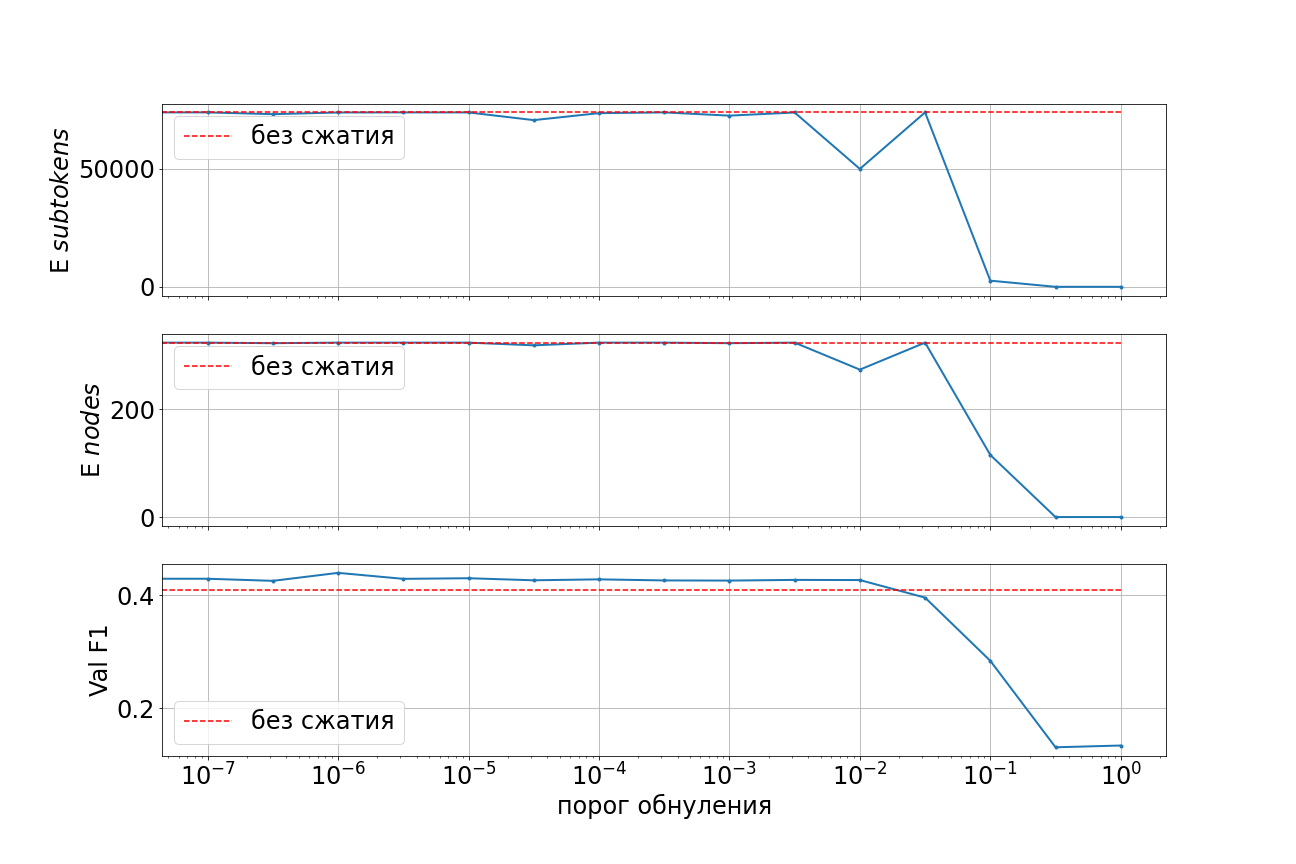
\includegraphics[width=0.8\textwidth]{example.png}
% 	\caption{Пример графика. Тут должна быть подпись, поясняющая что происходит на рисунке (краткая, но достаточная для понимания основной идеи графика).}
% 	\label{fig:by_epochs}
% \end{figure}

% Все рисунки в тексте должны иметь подписи и вы на них должны ссылаться в тексте. Например, на Рисунке~\ref{fig:by_epochs} изображен пример графика. Не забывайте подписывать все оси на графиках, добавлять легенду и пояснять все обозначения, а также используйте адекватного размера шрифты и толщину линий на графиках (все должно быть видно и понятно без многократного увеличения). На рисунке из примера явно не хватает обозначения синей линии в легенде.


% \subsection{Таблицы}

% Все таблицы в тексте тоже должны иметь подписи и вы на них должны ссылаться в тексте. Например, в Таблице~\ref{table:long_epochs} показаны результаты примерного эксперимента. 


% \begin{table}[ht]
% 	\caption{Пример таблички. Тут должна быть подпись, поясняющая что происходит в таблице (краткая, но по делу).}
% 	\label{table:long_epochs}
% 	\footnotesize
% 	\centering
% 	\begin{tabular}{lrrrrrrrr}
% 		\toprule
% 		& \multicolumn{3}{c}{$\mathsf{Val}$} &
% 		\multicolumn{3}{c}{$\mathsf{Test}$} \\
% 		\cmidrule(lr){2-4} \cmidrule(l){5-7} 
% 		{} &  $\mathsf{Prec}$ &  $\mathsf{Rec}$ &  $\mathsf{F1}$ &  $\mathsf{Prec}$ &  $\mathsf{Rec}$ &  $\mathsf{F1}$  &  $\mathsf{nodes}$ & $\mathsf{subtokens}$\\
% 		\midrule
% 		запуск 1    &    0.4894 &   0.3775 &  0.4263 &     0.4824 &    0.3683 &   0.4177 & 10029 & 179\\
% 		запуск 2    &    0.4887 &   0.3739 &  0.4237 &     0.4891 &    0.3724 &   0.4228 & 10039 & 177\\
% 		запуск 3    &    0.4820 &   0.3751 &  0.4219 &     0.4838 &    0.3677 &   0.4178 & 10037&	180\\
% 		\midrule
% 		\bf{среднее} &    \bf{0.4867} &   \bf{0.3755} &  \bf{0.4239} &    \bf{ 0.4851} &    \bf{0.3695} &   \bf{0.4195} \\
% 		\bf{дисперсия}  &    0.0041 &   0.0019 &  0.0022 &     0.0036 &    0.0025 &   0.0029 \\
% 		\bottomrule
% 	\end{tabular}
% \end{table}

% \subsection{Формулы}

% Формулы стоит центрировать, а также нумеровать, если вы ссылаете на них в тексте. Также не забывайте пояснять все обозначения в формулах. Например, запишем следующую задачу оптимизации:
% \begin{equation}
%     \label{eq:si_opt}
%         \theta* = \min_{\theta} F(\theta),
% \end{equation}
% где $F$~-- квадратичная функция от параметра $\theta$. При необходимости, далее в тексте можно сослаться на формулу~(\ref{eq:si_opt}). При этом, в зависимости от конкретных формул, можно использовать разные слова: формула, уравнение, задача оптимизации и т.п.


% \begin{thebibliography}{0}
% 	\bibitem{chirkova18}\hypertarget{chirkova18}{}
% 	\href{https://arxiv.org/abs/1810.10927}
% 	{Nadezhda Chirkova, Ekaterina Lobacheva, Dmitry Vetrov. Bayesian Compression for Natural Language Processing. In EMNLP 2018.}
% \end{thebibliography}
	
	
\end{document}
